\section{Positioning Game Counters}

This chapter describes how the map hexes are utilized to position counters during play. The game map is used to show exactly where aircraft, missiles, and other units, are located in relationship to each other. Every game counter must be placed on the maps so that its position is clear to all players.

\subsection{Basic Elements of Position}

\paragraph{Aircraft and Missile Counters.} Each aircraft and missile counter has a position which is defined by its map location, facing, and altitude.

\begin{itemize}
    \item \itemparagraph{Map Location.} With respect to the hexgrid, aircraft and missiles may be located wholly within a hex or on one of the lines between two hexes (commonly called a hexside). When located on a hexside, the game counter must face parallel to that hexside as illustrated \changedin{1D}{AWF}{below}{in Figure~\ref{figure:map-location}}. \addedin{1B}{JDW in the TSOH errata}{When determining range when one or both aircraft are on hexsides, count only the full hexes between them. Take the shortest number of hexes.}

    \changedin{1D}{AWF}{
    \begin{figure}[!ht]
    \centering
    \includegraphics[width=0.7\linewidth]{figures/figure-map-location.pdf}
    \end{figure}
    }{
    \begin{figure}
    \centering
    \begin{tikzfigure}{0.5\linewidth}
    \drawhexgrid{5}{3}  
    \drawaircraftcounter{2.00}{2.00}{90}{F-4}{}
    \drawaircraftcounter{1.50}{0.75}{120}{F-4}{}
    \drawaircraftcounter{4.00}{1.50}{90}{F-4}{}
    \miniathex{1.00}{1.50}{\node {\scriptsize Legal};}
    \miniathex{4.00}{2.20}{\node {\scriptsize Illegal};}
\end{tikzfigure}


    \caption{\protect\x{Map Location.}{Counters representing aircraft and missiles may be located wholly within a hex or on a hexside. When located on a hexside, the game counter must face parallel to that hexside.}}
    \label{figure:map-location}
    \end{figure}
    }

    \item \itemparagraph{Facing.} This is the horizontal direction in which an aircraft or missile is flying. Use the silhouette on the counter to show facing by pointing the nose of the aircraft or missile in one of the twelve possible directions. Each direction differs by 30 degrees and has a corresponding compass heading associated with it (i.e., N = North, SSE = South South-East, etc.). In the scenario booklets, next to the map layout diagrams, there will be a compass arrow indicating which direction relative to the hexgrid that is North. \changedin{1D}{AWF}{See diagram below.}{See Figure~\ref{figure:facing}.}

    \changedin{1D}{AWF}{
    \begin{figure}[!ht]
    \centering
    \includegraphics[width=0.7\linewidth]{figures/figure-facing.pdf}
    \end{figure}
    }{
    \begin{figure}
    \centering
    \begin{fitwidth}{0.7\linewidth}
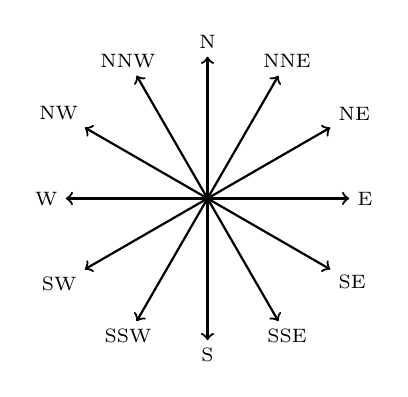
\begin{tikzpicture}
    \scriptsize
    \drawhex{0}{0}  
    \drawhex{0}{+1}  
    \drawhex{0}{-1}  
    \drawhex{+1}{+0.5}  
    \drawhex{+1}{-0.5}  
    \drawhex{-1}{+0.5}  
    \drawhex{-1}{-0.5}  
    \begin{scope}[thick,->]
        \draw (0,0) -- (0:1.8) node [anchor=180] {E};
        \draw (0,0) -- (30:1.8) node [anchor=210] {NE};
        \draw (0,0) -- (60:1.8) node [anchor=240] {NNE};
        \draw (0,0) -- (90:1.8) node [anchor=270] {N};
        \draw (0,0) -- (120:1.8) node [anchor=300] {NNW};
        \draw (0,0) -- (150:1.8) node [anchor=330] {NW};
        \draw (0,0) -- (180:1.8) node [anchor=0] {W};
        \draw (0,0) -- (210:1.8) node [anchor=30] {SW};
        \draw (0,0) -- (240:1.8) node [anchor=60] {SSW};
        \draw (0,0) -- (270:1.8) node [anchor=90] {S};
        \draw (0,0) -- (300:1.8) node [anchor=120] {SSE};
        \draw (0,0) -- (330:1.8) node [anchor=150] {SE};
    \end{scope}
    \drawaircraftcounter{0}{0}{60}{F-4}{}
\end{tikzpicture}
\end{fitwidth}


    \caption{\protect\x{Facing.}{The facing of an aircraft or missile is indicated by the direction of its nose on the game counter. The aircraft in the diagram is facing NNE.}}
    \label{figure:facing}
    \end{figure}
    }

    \item \itemparagraph{Altitude.} An aircraft or missile's altitude is kept track of on the aircraft's log sheet in terms of numbered levels. Each altitude level represents 1000 feet of height thus the number of a level corresponds to the altitude in thousands of feet (i.e., level 24 = 24,000 feet). Altitude levels are further grouped into named bands as described later in the rules. Aircraft and missile performance may vary in each altitude band as shown on an aircraft's data card and in the missile flight tables.

\end{itemize}

\paragraph{Ground and Naval Unit Counters.} Ground combat units and naval units have their positions defined simply by map location. They are always placed wholly within hexes and never on hexsides. Ground units never consider facing\addedin{1B}{JDW in the TSOH errata}{ (except heavy AAA units under advanced rule 24.5)}, but large naval units must be faced in specific directions as for aircraft and missiles.

\subsection{Stacking}

It is allowed, within the limits given below, for more than one counter to be in the same position on the map at the same time. When counters end up on top of other counters at the end of a turn, they are considered stacked. Stacking restrictions apply only al the end of a turn after all moves are completed.

\paragraph{In The Air.} Aircraft and missiles may freely fly through hexes or hexsides containing other game counters. They may freely stack on top of ground and naval units. They may freely stack with other aircraft and missiles that are not at the same altitude level. However, no more than two friendly aircraft may safely end up stacked together at the same altitude level (unless in Close Formation). Aircraft from opposing sides may not stack together at the same altitude safely. If these last two situations occur, you must check for collisions.

Exception: Up to four aircraft may be stacked together and may safely fly together at the same altitude while in a close formation. See advanced Rule 5.6.

\paragraph{On The Ground.} No more than four ground unit counters may ever stack in the same ground terrain hex. No more than four small naval unit counters may ever stack in the same water, coastal, or river terrain hex. No more than two large naval unit counters may ever stack in the same water hex. When taxing on the ground, up to four aircraft may move together in a stack.

\subsection{Aircraft Collisions}

Collisions are possible during the Flight Phase whenever an aircraft executes a head-on gun attack at range zero\addedin{1C}{FH in APJ 36}{ and the aircraft are at the same altitude}. Collisions are also possible at the end of \changedin{1C}{FH in APJ 36}{a game-turn}{the flight phase} in the following situations:

\begin{itemize}
    \item If an aircraft is stacked at the same altitude level with any enemy aircraft, and/or
    \item If an aircraft is stacked with two or more friendly aircraft and not in Close Formation.
\end{itemize}

\paragraph{Collision Resolution:} For each potential collision, the player who last moved into the position must roll the die. On a roll of 1, his aircraft collides with one of the others. Determine which aircraft it collides with randomly. Both aircraft immediately roll on the 10 column of the Damage table to determine their damage.

\paragraph{Collision Exceptions:} There are \changedin{1C}{FH in APJ 36}{two}{three} exceptions to the Potential Collision rule.

\begin{itemize}
    \item An aircraft tailing another will not collide with that aircraft.
    \item An aircraft which is flying in close formation will not collide with other friendly aircraft in that formation.
    \itemaddedin{1C}{FH in APJ 36}{An aircraft that have already rolled for a collision for a head-on gun attack does not roll again for a collision again at the end of the flight phase.}
\end{itemize}

\notein{1B}{There is a clarification of the collision exceptions in the TSOH errata, but it seems to restate the original exceptions. I have not included it.}

